\documentclass[11pt, dvipdfmx]{beamer}
%\documentclass[8,9,10,11,12,14,17,20pt, dvips, handout]{beamer}
%%%%%%%%%%%  package  %%%%%%%%%%%
\usepackage{amssymb,amsmath,ascmac}
\usepackage{atbegshi}

\AtBeginShipoutFirst{\special{pdf:tounicode 90ms-RKSJ-UCS2}}
\usepackage{minijs}
\renewcommand{\kanjifamilydefault}{\gtdefault}
\usepackage{multirow}
\usepackage{bm}

\usepackage{tikz}
\usepackage{xparse}
\usetikzlibrary{shapes,arrows}
%% define fancy arrow. \tikzfancyarrow[<option>]{<text>}. ex: \tikzfancyarrow[fill=red!5]{hoge}
  \tikzset{arrowstyle/.style n args={2}{inner ysep=0.1ex, inner xsep=0.5em, minimum height=2em, draw=#2, fill=black!20, font=\sffamily\bfseries, single arrow, single arrow head extend=0.4em, #1,}}
  \NewDocumentCommand{\tikzfancyarrow}{O{fill=black!20} O{none}  m}{
    \tikz[baseline=-0.5ex]\node [arrowstyle={#1}{#2}] {#3 \mathstrut};}

%微分関連のマクロ
%
\newcommand{\diff}{\mathrm d}
\newcommand{\difd}[2]{\dfrac{\diff #1}{\diff #2}}
\newcommand{\difp}[2]{\dfrac{\partial #1}{\partial #2}}
\newcommand{\difdd}[2]{\dfrac{\diff^2 #1}{\diff #2^2}}
\newcommand{\difpp}[2]{\dfrac{\partial^2 #1}{\partial #2^2}}

\renewcommand\appendixname{Appendix}

\graphicspath{{../Figures/Rheology/}{../Figures/adhesives/}}

%%%%%%%%%%%  theme  %%%%%%%%%%%

%%%%%
% Simple
%%%%%
%\usetheme{default}
%\usetheme{Pittsburgh}
%\usetheme{Rochester}
%\usetheme{Szeged}

%%%%%
% So So
%%%%%
%\usetheme{Singapore}
%\usetheme{CambridgeUS}
\usetheme{Copenhagen}
%\usetheme{Luebeck}
%\usetheme{Malmoe}
%\usetheme{Warsaw}

%%%%%
% No Heasder
%%%%%
%\usetheme{Madrid}
%\usetheme{Boadilla}

%%%%%
% No Footer
%%%%%
%\usetheme{Darmstadt}
%\usetheme{JuanLesPins}
%\usetheme{Montpellier}

%%%%%
% Color
%%%%%
%\usetheme{AnnArbor}

%%%%%
% Too much
%%%%%
%\usetheme{Berlin}
%\usetheme{Ilmenau}

%%%%%
% Right hand Side
%%%%%
%\usetheme{Goettingen}
%\usetheme{Marburg}

%%%%%
% Left hand Side
%%%%%
%\usetheme{PaloAlto}


%%%%%%%%%%%  inner theme  %%%%%%%%%%%
\useinnertheme{default}
%\useinnertheme{circles}
%\useinnertheme{inmargin}
%\useinnertheme{rectangles}
%\useinnertheme{rounded}


%%%%%%%%%%%  outer theme  %%%%%%%%%%%
\useoutertheme{default}


%%%%%%%%%%%  font theme  %%%%%%%%%%%
\usefonttheme{professionalfonts}
%\usefonttheme{default}
%\usefonttheme{serif}
%\usefonttheme{structurebold}
%\usefonttheme{structureserif}
%\usefonttheme{structuresmallcapsserif}


%%%%%%%%%%%  degree of transparency  %%%%%%%%%%%
%\setbeamercovered{transparent=30}

%\setbeamercolor{item}{fg=red}
\setbeamertemplate{items}[default]

%%%%%%%%%%%  numbering  %%%%%%%%%%%
%\setbeamertemplate{numbered}

\setbeamertemplate{navigation symbols}{}
%%%%%%%%%%%%%%%%%%%%%%%%%%%%%%%%%%%
\title
[高分子材料の破壊について]
{高分子材料の破壊について}
\author[佐々木]{佐々木裕}
% \institute[東亞合成]{東亞合成}
\date{\today}
%%%%%%%%%%%%%%%%%%%%%%%%%%%%%%%%%%
\begin{document}
%%%%%%%%%%%%%%%%%%%%%%%%%%%%%%%%%%
\begin{frame}\frametitle{}
	\titlepage
\end{frame}

\section{高分子材料の破壊}
%%%%%%%%%%%%%%%%%%%%%%
%%%%%%%%%%%%%%%%%%%%%%%%%%%%
\subsection{高分子材料への期待と不安:耐久性}
%%%%%%%%%%%%%%%%%%%%%%%%%%%%
\begin{frame}
\frametitle{高分子材料への期待と不安}
{\Large
地球温暖化対策の CO$_2$ 削減へ向けて、\\
{\color{red}「自動車を中心とした運送機器の抜本的な軽量化」}
\\
が提唱されている。}

\begin{block}{高分子材料への期待}
	\begin{itemize}
	\item
	現行の鉄鋼主体$ \Rightarrow$ 高分子材料を含むマルチマテリアル化
	
	\item
	高分子材料によるマルチマテリアル化のポイント
		\begin{itemize}
		\item
		高い比強度の有効利用
		\item
		特徴を生かした適材適所 $\Leftrightarrow$ 適切な接合方法の選択
			\begin{itemize}
			\large
			\item
			{\color{red} 「接着接合」への高分子の利用}
			\item
			{\color{red} 「柔らかさを生かした弾性接着接合」}
			\end{itemize}
		\Large
		\item
		{\color{blue}耐久性が不明確(特に疲労破壊に対して)}
		\end{itemize}
	\end{itemize}
\end{block}
\normalsize
\end{frame}

%%%%%%%%%%%%%%%%%%%%%%%%%%%%%%%%
\subsection{固体バルクの力学応答}
%%%%%%%%%%%%%%
\begin{frame}
\frametitle{一般的な応力 - 歪み曲線}

\begin{columns}[totalwidth=1\textwidth]
\column{.6\textwidth}
	\begin{itemize}
	\item 線形領域(~弾性限界):
		\begin{itemize}
		\item この段階までの変形は可逆
		\item {\color{red}「内部構造は変化しない」}
		\end{itemize}
	\item 弾性限界から降伏点:
		\begin{itemize}
		\item 直線から外れて応力が極大
		\item {\color{blue}「不可逆な内部構造の変化が\\生じはじめる」}
		\end{itemize}
	\item 降伏点以降:
		\begin{itemize}
		\item 塑性変形が進行し、破断
		\item 破断点近傍で、{\color{red}「局所的な高分子鎖の切断$\Rightarrow$マクロな破壊」}
		\end{itemize}
	\end{itemize}
%}
\column{.39\textwidth}
%\vspace{-20mm}
	\begin{figure}
	\centering
	
\includegraphics[width=50mm]{S_S_Curve.png}
	\end{figure}
\end{columns}
\end{frame}
%%%%
\subsection{破壊のモード}
\begin{frame}
\frametitle{脆性破壊と延性破壊}

\begin{columns}[totalwidth=1\textwidth]
\column{.5\textwidth}
	\begin{itemize}
	\item 脆性破壊:
		\begin{itemize}
		\item 
		弾性限界を超えると、
		\item
		巨視的な亀裂が生じ、
		\item
		分離し破壊
		\end{itemize}
	\item 延性破壊:
		\begin{itemize}
		\item 
		降伏点が存在し、
		\item
		降伏歪以上でも、
		\item
		延性を示す
		\end{itemize}
	\end{itemize}
%}
\column{.49\textwidth}
%\vspace{-20mm}
	\begin{figure}
	\centering
	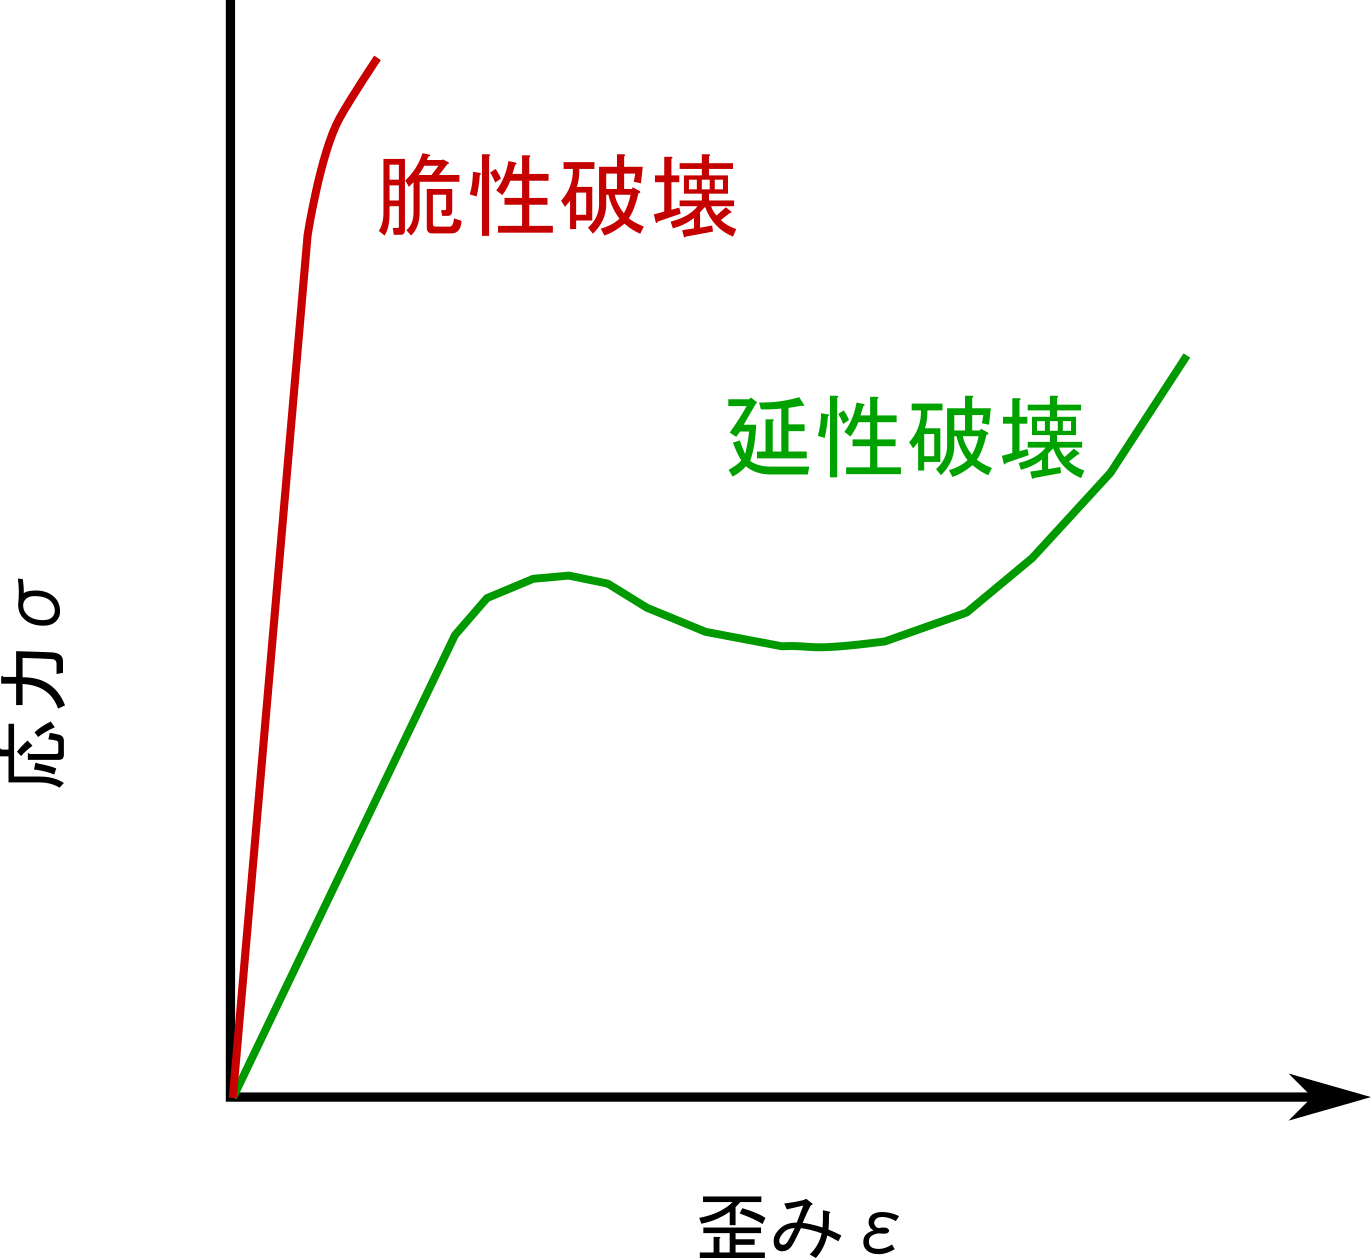
\includegraphics[width=50mm]{S_S_Curve_2.png}
	\end{figure}
\end{columns}

\begin{description}
\item[塑性変形]
弾性限界を超えた外力の印加により生じた歪みのうち、除荷後にも残る永久歪み。
\item[脆性および延性破壊]
主として、塑性変形時に発生する破壊。
\end{description}
\end{frame}

\section{破壊工学の考え方}

\subsection{Griffith 理論}
\begin{frame}
	\frametitle{応力集中係数}

	楕円状欠陥の応力集中は以下のように書ける。
\begin{align}
&\sigma_{max} = \sigma_0 \left( 1+2\sqrt{\dfrac{c}{\rho}} \right) \notag \\[8pt]
&2c:\;\text{楕円状欠陥の全長} \notag \\
&\rho:\;\text{欠陥先端の曲率半径}
\end{align}
この $\sigma_0$ への係数を「応力集中係数」とよぶ。

亀裂においては、欠陥の先端が先鋭化し $\rho \rightarrow 0$ となるので、応力集中係数も無限大に発散してしまうことになる。


\end{frame}
\begin{frame}
	\frametitle{Griffith 理論}

	グリフィスは、亀裂(長さ $2c$)により解放されるひずみエネルギーと、亀裂表面の表面エネルギーが平衡を保つと仮定し、亀裂成長の条件を以下のように導いた。
\begin{align}
\dfrac{\pi c^2 \sigma^2}{E} \geq 2 \gamma
\end{align}

この条件式はガラスのような脆性破壊を示す材料には適合する。

上式の左辺は、亀裂の進展により解放されるエネルギーを表すので、エネルギー開放率 $G$ と呼ぶ。

上記のグリフィスの条件は、理想的な線形材料の脆性破壊でない限り、$\gamma$ は表面エネルギーの値には対応しない。
実験的に求められる実際の材料においては、非線形性(塑性変形エネルギー等)が含まれている。
これを考慮して $\gamma_p$ とすれば、
\begin{align}
\dfrac{\pi c^2 \sigma^2}{E} \geq 2 (\gamma+\gamma_p)
\label{Gr}
\end{align}


\end{frame}

\subsection{破壊工学の考え方}
%%%%%%%%%%%%%%%%%%%%%%%%%%%%%%
\begin{frame}
\frametitle{破壊工学の考え方}
\begin{exampleblock}{系中にクラックが存在することを前提に}

\begin{itemize}
\item
\alert{「クラック近傍での応力集中を如何に抑制するか」}
\end{itemize}
\end{exampleblock}

\begin{columns}[totalwidth=1\textwidth]
\column{.5\textwidth}
\begin{alertblock}{マクロとミクロをつなげると}
	\begin{itemize}
		\item
		\alert{応力拡大係数 $K_I$ で評価}
		\small
		\begin{align*}
		K_{I} = \sigma \sqrt{\pi c}
		\end{align*}
		\normalsize
		\item 
		クラック進展の抑制 \\
		$\Rightarrow$ 先端での\alert{局所降伏}\\
		降伏応力 $\sigma_Y$ に反比例
		\small
		\begin{align*}
		d \propto \left( \dfrac{K_I}{\sigma_Y} \right)^2
		\end{align*}
		\normalsize
	\end{itemize}
\end{alertblock}
\column{.5\textwidth}
	\centering
	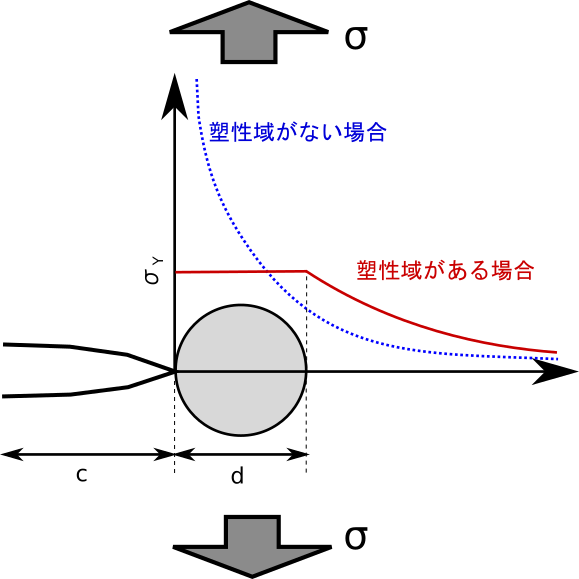
\includegraphics[width=.9\textwidth]{yeild_crack.png}
\end{columns}
\end{frame}

\subsection{高分子の破壊}
%%%%%%%%%%%%%%%
\begin{frame}
%[shrink squeeze]
\frametitle{降伏挙動と破壊モード}
\begin{columns}[totalwidth=1\textwidth]
\column{.5\textwidth}
ガラス状態の高分子材料では、
\begin{block}{破壊のモード(巨視的)}
脆性破壊 $\Leftrightarrow$ 延性破壊\\
脆性破壊は、降伏前にミクロなクラックが進展した破壊とも考えられる。
\end{block}
\column{.5\textwidth}
	\centering
	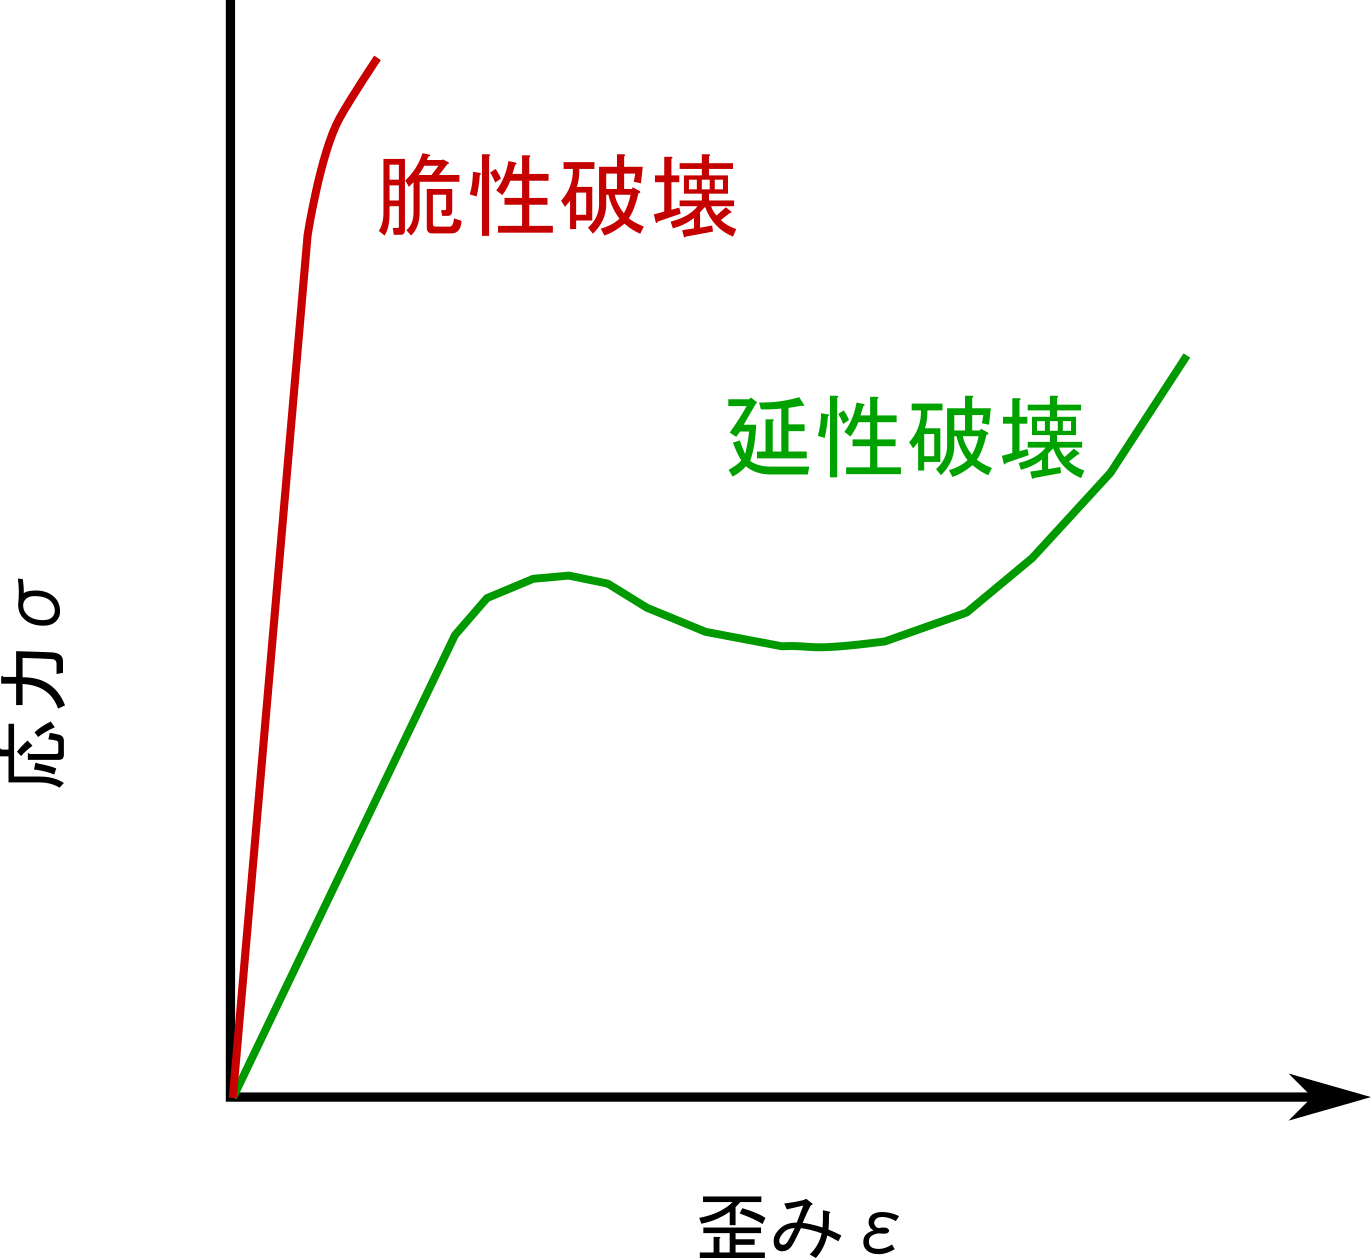
\includegraphics[width=.9\textwidth]{S_S_Curve_2.png}
\end{columns}
\begin{exampleblock}{延性破壊モードにするために}
	\begin{itemize}
		\item
		{\color{red} 局所的な降伏}が必須。
		\item
		クレイズのような局所的な破壊も含む
		\item 
		一般に、高分子材料の{\color{red} 降伏は不可逆}。
	\end{itemize}
\end{exampleblock}
\end{frame}




%%%%%%%%%%%%%%%%%%%%%%
\section{破壊と粘弾性}
\subsection{ゴムの強靭性}
%%%%%%%%%%%%%%%%%%%%%%
\begin{frame}
\frametitle{ゴムの強靭性}


\begin{columns}[totalwidth=1\textwidth]
\column{.6\textwidth}
\begin{exampleblock}{Andrews 理論}
クラック先端の応力の等高線表示
	\begin{itemize}
	\item
	クラック成長時の応力場の考察より、
		\begin{itemize}
		\item
		{\color{red} Loading 場とUnloading 場の差}が重要。
		\item
		この差は\alert{ヒステリシスに由来}
		\end{itemize}	
	\item
	\alert{ひずみエネルギー開放率が低減} \\$\Rightarrow$ 強靭さの起源。
	\end{itemize}
\end{exampleblock}

{Andrews, E. H. and Fukahori, Y., Journal of Materials Science, 12, 1307 (1977)}

\column{.4\textwidth}
\centering
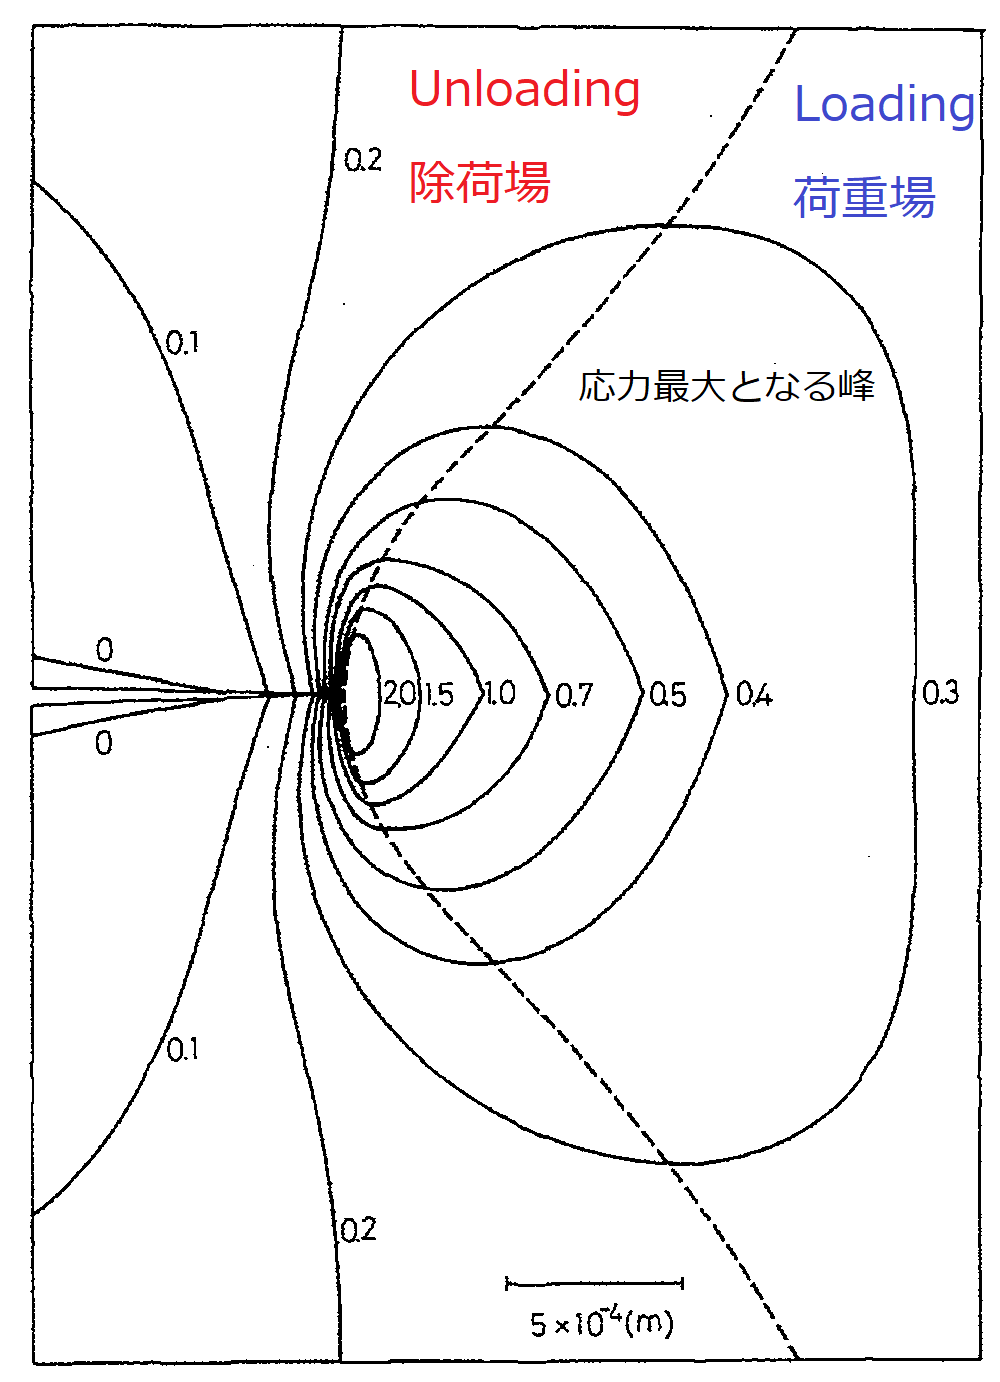
\includegraphics[width=40mm]{./fig/crack.png}
\end{columns}
\end{frame}

\subsection{ゴムの破壊と粘弾性}
%%%%%%%%%%%%%%%%%
\begin{frame}
    \frametitle{ゴムの破壊と粘弾性}
    
    \vspace{-2mm}
    \begin{alertblock}{ゴムの破壊}
    大変形を伴う非線形現象だが、時間温度換算則の成立が多数報告
    \end{alertblock}
    
    \begin{columns}[totalwidth=1\textwidth]
    \column{.48\textwidth}
    ゴムの亀裂先端近傍での大変形
    \centering
    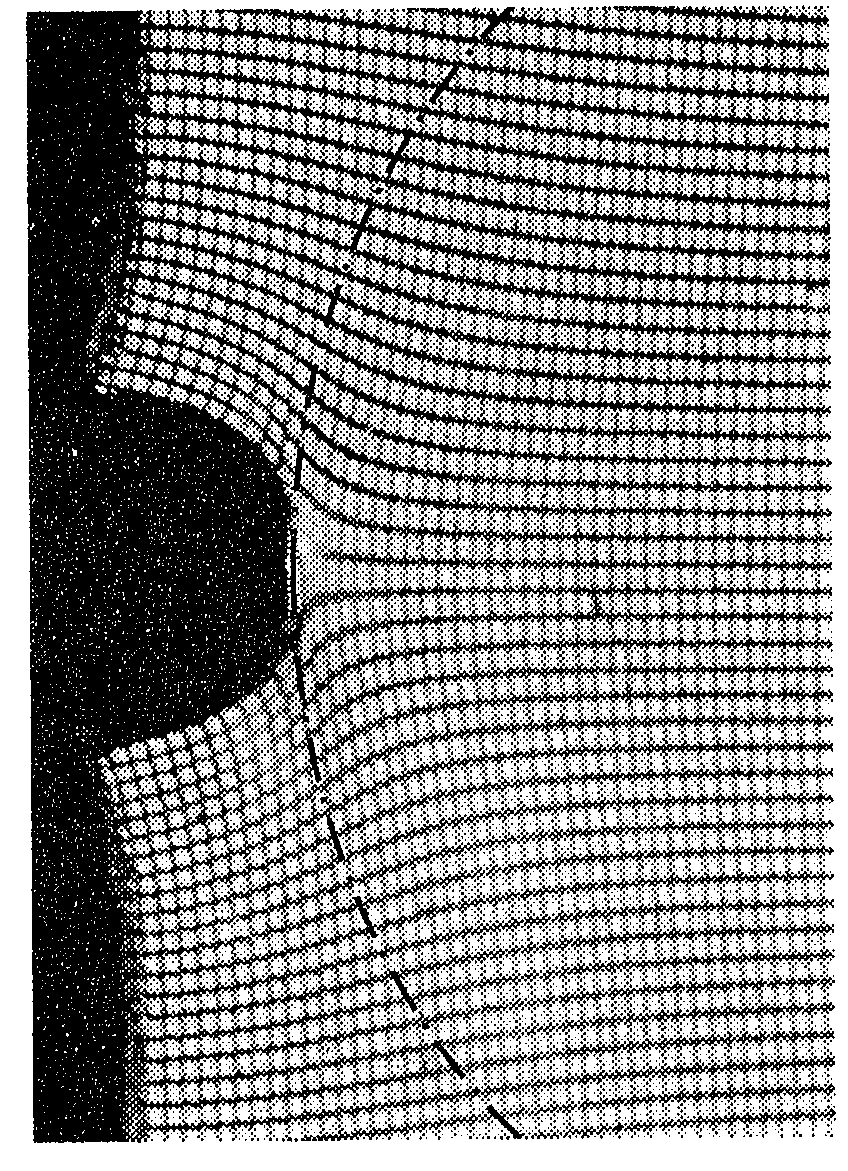
\includegraphics[width=.7\textwidth]{./fig/rubber_crack.png}
    \column{.48\textwidth}
    時間温度換算則の成立
    \centering
    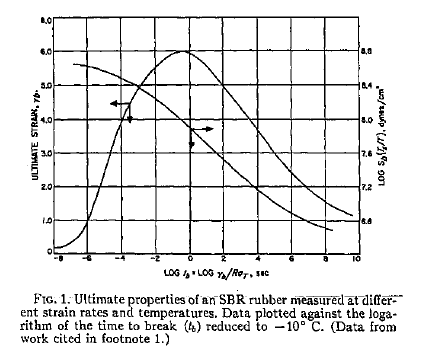
\includegraphics[width=\textwidth]{./fig/Time_Temp_2.png}
    
    {\tiny Smith T., Stedry P., J. Appl. Phys. (1960) 31 1892}
    
    \end{columns}
    \end{frame}

%%%%%%%%%%%%%%%%%
\begin{frame}
    \frametitle{SBRでの伸びきり効果}
    
    \centering
    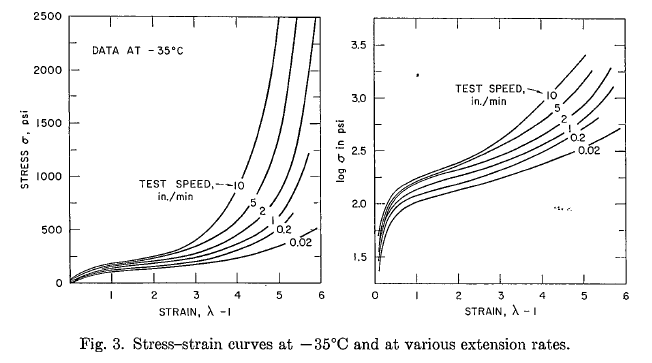
\includegraphics[width=8.5cm]{./fig/SBR_lowTemp_2.png}
    
    {\tiny Smith TL., Dickie RA., J. Pol. Sci. part A-2 (1969) 7 635}
    
    \begin{alertblock}{室温で伸び切りが出ないはずのSBR}
    \begin{itemize}
    \item
    低温、高速変形でSBRでも伸びきり効果が発現
    \item
    時間温度換算則で考えてみれば?
    \end{itemize}
    \end{alertblock}
    \end{frame}

    
\subsection{ネットワークポリマーについて}
%%%
\begin{frame}
    \frametitle{かつての実験結果}
    
    \begin{columns}[totalwidth=1\textwidth]
    \column{.5\textwidth}
    
    ``Constrained Junction model''
    
    \begin{itemize}
    \item
    未伸長時
        \begin{itemize}
        \item
        架橋点の揺らぎは抑制
        \item
        架橋点は ``Affine'' で変形
        \end{itemize}
    \item
    高延伸化
        \begin{itemize}
        \item
        鎖方向への拘束が緩和
        \item
        ``Phantom model'' に移行
        \end{itemize}
    \end{itemize}
    
    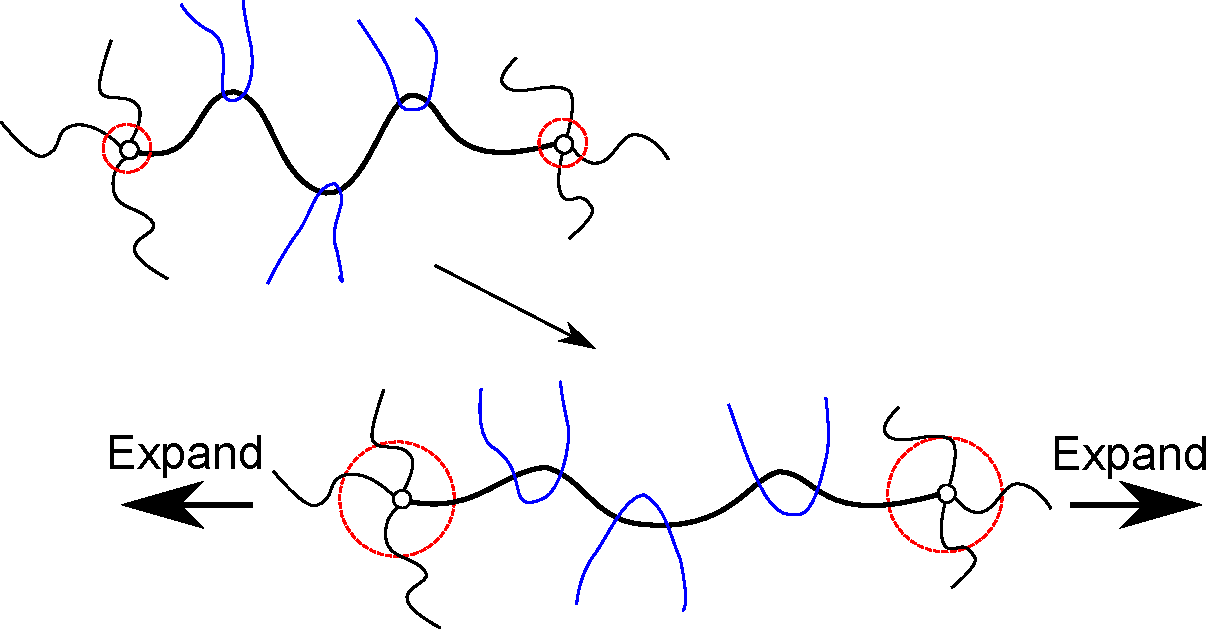
\includegraphics[width=\columnwidth]{./fig/Constrained_Juntion.pdf}
    
    \footnotesize
    P.J.Flory, J.C.P., 66, 5720 (1977)  
    
    %\pause
    \column{.5\textwidth}
    Flory のパラメタ($\kappa:$ 絡み合いによる拘束の度合い)ではなく、変形量に応じた緩和の形で、
    \scriptsize
    \begin{align*}
    \sigma_{fit}&=Gk\exp\left( -\dfrac{\lambda}{\tau} \right) (\lambda-1/\lambda^2)\\
    &\quad k\simeq0.85, \tau \simeq 5.7
    \end{align*}
    
    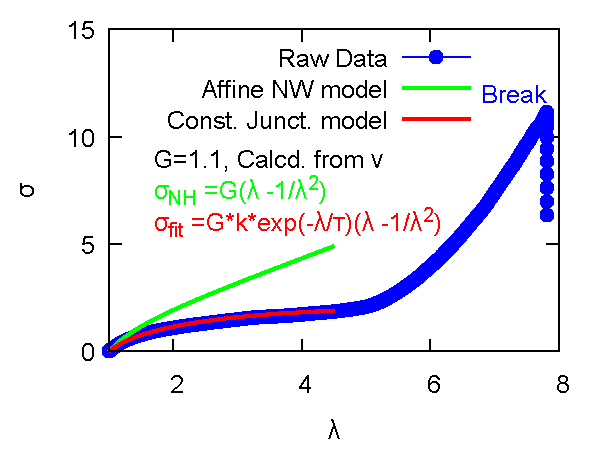
\includegraphics[width=\columnwidth]{./fig/SS_MR_6_fit.pdf}
    
    \end{columns}
    \end{frame}
    
    %%%%%%%%%%%%%%%%%%%%%%%%%%%%%%%%%%%%%%%%%%%%%%%%
    \begin{frame}
        \frametitle{架橋点近傍の拘束状態に基づく二つのモデル}
		\vspace{-3mm}
        \begin{columns}[totalwidth=1\textwidth]
        \column{.5\textwidth}
        ストランドと架橋点の模式図
        %\centering
        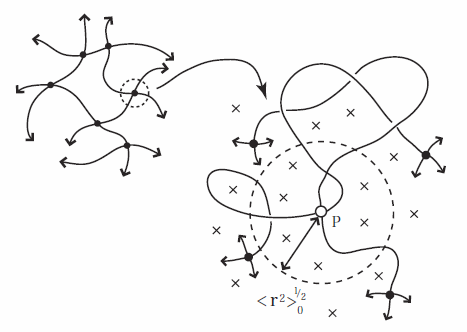
\includegraphics[width=\textwidth]{./fig/JP_vicinity.png}
        架橋点はストランド経由で直接連結した架橋点(図中の黒丸)以外の、近接する多数のストランド及び架橋点(図中の×)に囲まれている。
        \column{.5\textwidth}
        \begin{itemize}
        \item
        ``Affine NW Model''\\
        架橋点は周辺に強く拘束され巨視的変形と相似に移動。\\(Affine 変形)
        \footnotesize
        \begin{equation*}
        G=\nu k_B T
        \end{equation*}
        \normalsize
        $\nu$ は、ストランドの数密度
        \item
        ``Phantom NW Model''\\
        架橋点が大きく揺らぎ、実効的なずり弾性率($G$)が低下。
        \footnotesize
        \begin{align*}
        G&=\xi \nu k_B T \\
        \xi&= 1 -\dfrac{2}{f}
        \end{align*}
        \normalsize
        $f$ は架橋点の分岐数
        \end{itemize}
        \end{columns}
        \end{frame}

    %%%%%%%%%%%%%%%%%%%%%%%%%%%%%%%%%%%%%%%%%%%%%%%%
    \begin{frame}
        \frametitle{最近の結果(せん断変形)}
		\begin{itemize}
			\item 絡み合いの効果を排除して評価するために、末端間距離を自然長に設定したネットワークを一重で設定。
			\item 密度は、低い状態でシミュレート。
			\item 高温でのシミュレーションに相当
		\end{itemize}
		
        \begin{columns}[totalwidth=1\textwidth]
        \column{.5\textwidth}
        %\centering
        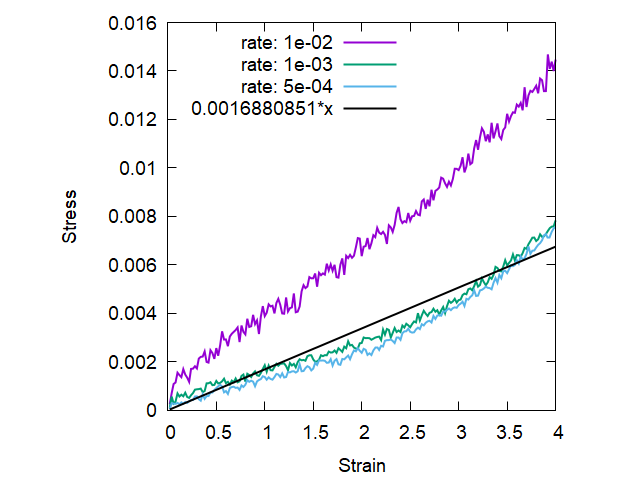
\includegraphics[width=\textwidth]{./fig/reg_4_SS_multi.png}
        
		RegularNW-4-chains-N50
        \column{.5\textwidth}
        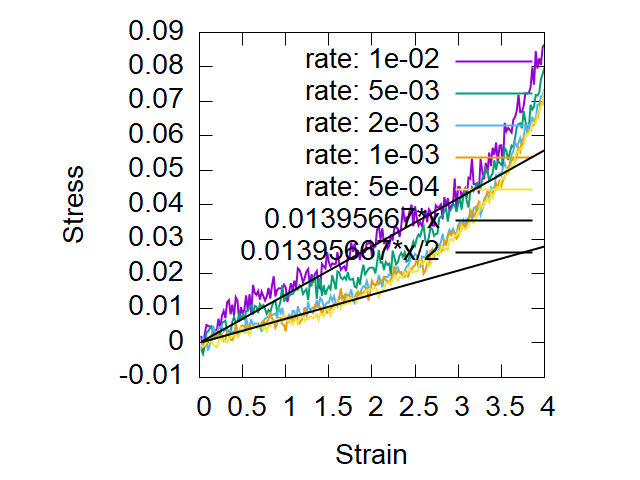
\includegraphics[width=\textwidth]{./fig/random-4chain-SS_multi.png}

		RandomNW-4-chains-N20
        \end{columns}
        \end{frame}
% %%%%%%%%%%%%%%%%%%%%%%%%%%
% \section{検討内容}
% %%%%%%%%%%%%%%%%%%%%%%%%%%
% %%%%%%%%%%%%%%%%%%
% %\begin{frame}
% %\LARGE{検討内容}
% %\end{frame}
% %%%%%%%%%%%%%%%%%%%%%%%%%%%%%%%%%
% \subsection{ランダムネットワーク構造の作成}
% %%%%%%%%%%%%%%%%%%%%%%%%%%
% \begin{frame}
% \frametitle{ランダムなネットワークの作成}
% \small
% \vspace{-2mm}
% \begin{block}{ここでのランダムの定義}
% \begin{itemize}
% \item
% ユニットセルの連なりとしてネットワークを考え、
% \item
% 各ユニットセルごとにその内部の接続性をランダムとする。
% \item
% これは、\alert{各ノードの隣接関係をランダム}にすることに対応。
% \end{itemize}
% \end{block}
% \vspace{-2mm}
% \begin{exampleblock}{アルゴリズム}
% \begin{enumerate}
% \item
% 初期構造の作成
% 	\begin{itemize}
% 	\item
% 	\alert{実空間}で8-Chain Model で初期構造を作成。
% 	\item
% 	所望の分岐数に\alert{ランダム}に選択した\alert{結合(エッジ)を除去}
% 	\item
% 	除去したジオメトリーに対応した\alert{トポロジーモデル}を作成
% 	\end{itemize}
% \item
% ランダム性の導入
% 	\begin{itemize}
%  	\item 
%  	ラプラシアン行列で\alert{全体の連結性を確認}しながら、
%  	\item
%  	エッジ交換して、ランダム性を導入
% 	\end{itemize}	
% \item
% トポロジーモデルに対応する実空間でのネットワーク初期構造作成
% \end{enumerate}
% %\color{red} こうすれば、実空間で遠く離れたノードをつなげることはない。
% \end{exampleblock}
% \end{frame}

% %%%%%%%%%%%%%%%%%%%%%%%%%%
% \begin{frame}
% \frametitle{トポロジーモデルへの変換}
% \begin{columns}[totalwidth=1\textwidth]
% \column{.48\textwidth}
% \begin{block}{実空間での初期構造}
% \small
% \begin{itemize}
% \item
% $2\times2\times2$ 個のユニットセル
% \vspace{-2mm}
% \begin{figure}
% \centering
% 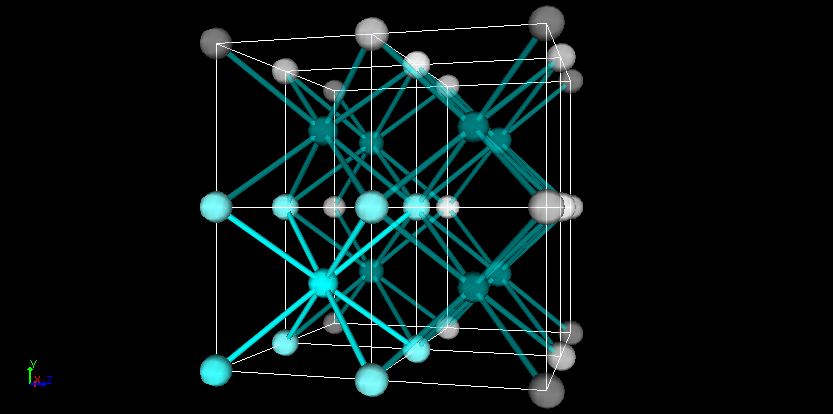
\includegraphics[width=0.8\columnwidth]{./fig/8_per.png}
% \end{figure}
% \vspace{-2mm}
% \item
% \vspace{-2mm}
% ユニットセルから除去
% \vspace{-2mm}
% \begin{figure}
% \centering
% 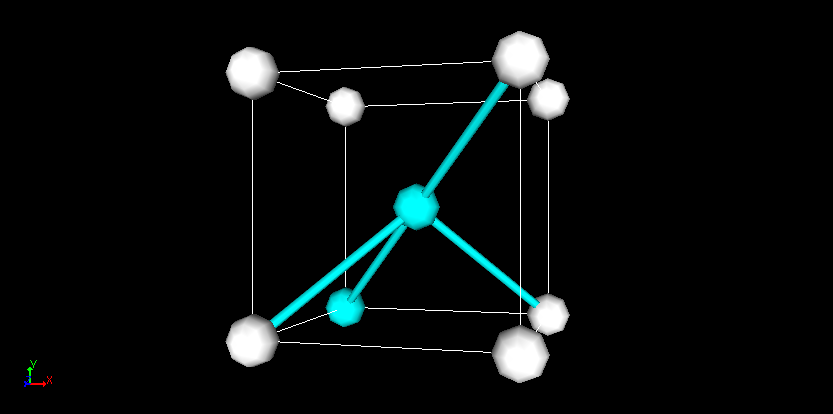
\includegraphics[width=0.8\columnwidth]{./fig/8_4.png}
% \end{figure}
% \end{itemize}
% \end{block}
% \column{.48\textwidth}
% \begin{exampleblock}{トポロジーモデル}
% \small
% 分岐数を4に減じたトポロジーモデル
% \vspace{-2mm}
% \begin{figure}
% \centering
% 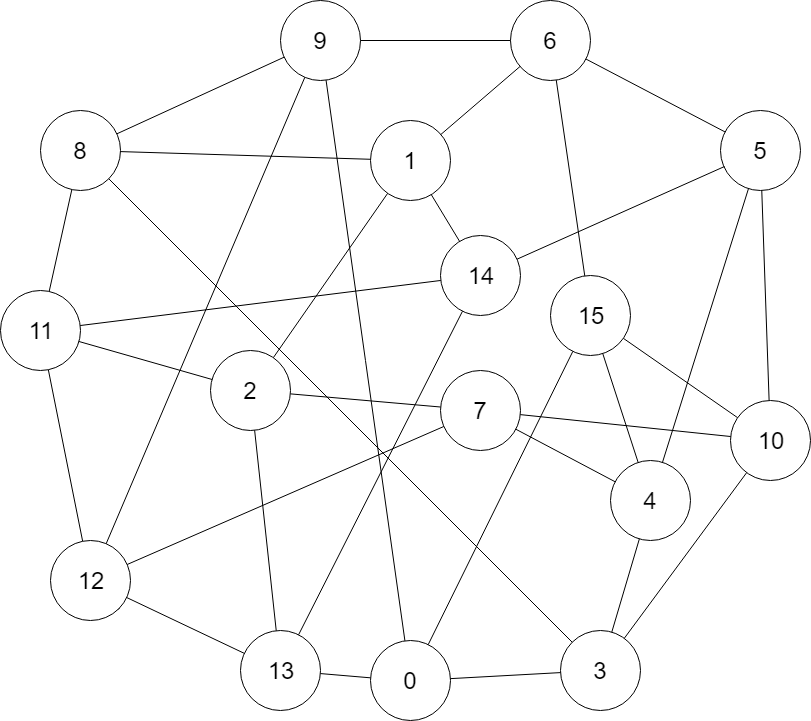
\includegraphics[width=\columnwidth]{./fig/Network.png}
% \end{figure}
% \end{exampleblock}
% \end{columns}
% \end{frame}

% %%%%%%%%%%%%%%%%%%%%%%%%%%
% \begin{frame}
% \frametitle{トポロジーモデルからのランダム性の導入}

% \vspace{-8mm}
% \begin{figure}
% \centering
% 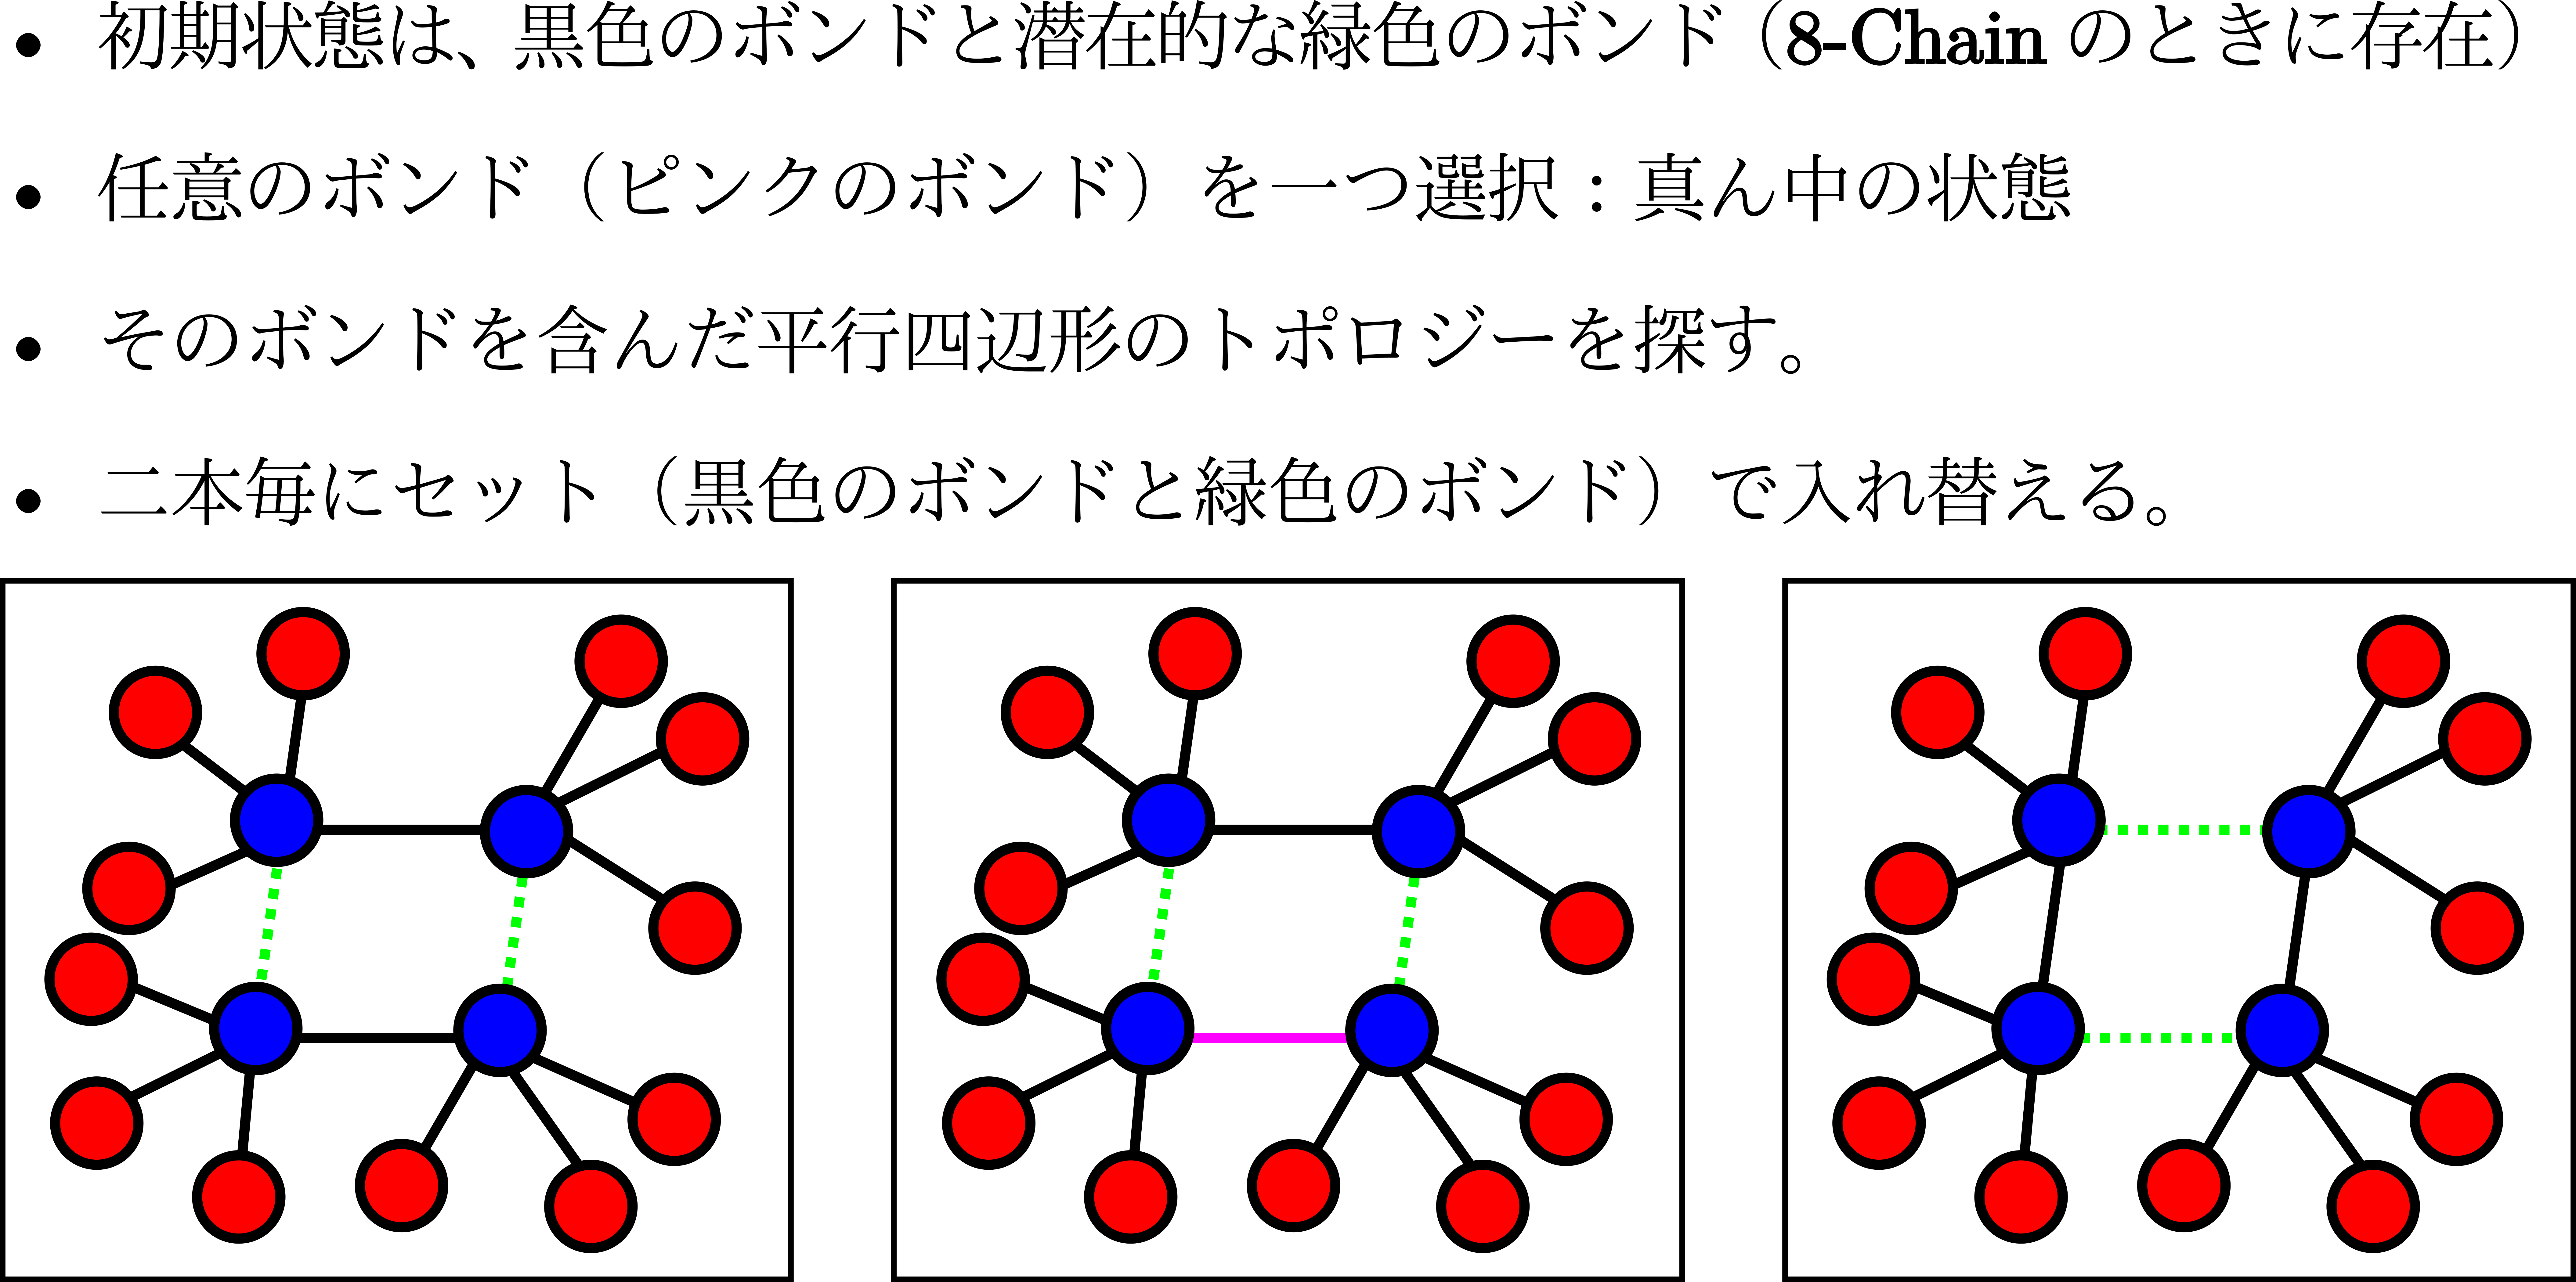
\includegraphics[width=11cm]{./fig/ボンド交換.png}
% \end{figure}
% \end{frame}



% %%%%%%%%%%%%%%
% \begin{frame}
% \frametitle{ファントムネットワークのゆらぎ}

% \begin{columns}[totalwidth=1\textwidth]
% \column{.47\textwidth}
% \scriptsize
% \begin{block}{ゆらぎの入ったポテンシャル}
% ストランドの末端間ベクトル $\bm{R}_{nm}$ を、\\架橋点の位置ベクトル $\bm{r}_n$ を用いて、
% \vspace{-3mm}
% \begin{equation*}
% \bm{R}_{nm} \equiv \bm{r}_n-\bm{r}_m
% \end{equation*}

% 系のポテンシャルエネルギーは、
% \vspace{-3mm}
% \begin{equation*}
% U=\dfrac{k}{2} \sum_{\langle nm \rangle} \bm{R}_{nm}^2
% \end{equation*}

% これは、自然長で決まる定数項と、ゆらぎに起因した第二項に分割でき、その和で以下となる。
% \vspace{-3mm}
% \begin{equation*}
% U=\dfrac{k}{2} \sum_{\langle nm \rangle} {\bm{R}_{nm}^{(0)}}^2 + \dfrac{k}{2} \sum_{\langle nm \rangle} \Delta \bm{R}_{nm}^2
% \end{equation*}
% \end{block}

% \column{.47\textwidth}
% \scriptsize
% \begin{block}{アンサンブル平均の二つの表式}
% \vspace{-5mm}
% \begin{align*}
%  \begin{cases}
% 	\langle U \rangle = N_{strands} \dfrac{k}{2} \langle \Delta \bm{R}^2 \rangle \\
% 	\langle U \rangle = 3(N_{nodes}-1) \dfrac{1}{2} k_B T
%  \end{cases}
% \end{align*}
% なお、第二式は等分配側より導出した。
% \end{block}

% \begin{exampleblock}{ファントムネットワークでのゆらぎ}
% 架橋点数 $N_{nodes}$、架橋点官能基数 $f$ とすれば、規則格子での一般式として、
% \vspace{-3mm}
% \begin{equation*}
% \langle \Delta \bm{R}^2 \rangle = \dfrac{3k_B T}{k} \dfrac{2}{f} \left( 1-\dfrac{1}{N_{nodes}} \right)
% \end{equation*}

% 適切な条件で、ストランドの自然長 $R_0$\\
% を用いて、
% \vspace{-3mm}
% \begin{equation*}
% \color{red}
% \langle \Delta \bm{R}^2 \rangle = \dfrac{2}{f} R_0^2
% \end{equation*}
% \vspace{-6mm}
% \end{exampleblock}

% \end{columns}

% \end{frame}



% %%%%%%%%%%%%%%%%%%%%%%%%%%
% \begin{frame}
% \frametitle{ファントムネットワークモデルの有限サイズ効果}
% \begin{columns}[totalwidth=1\textwidth]
% \column{.48\textwidth}
% \begin{block}{壁面に末端が固定された効果}
% \begin{itemize}
% \item
% 壁面に末端が固定
% 	\begin{itemize}
% 	\item  
% 	$n$ 本のストランド
% 	\item
% 	セグメント数: $N$
% 	\item
% 	他端が架橋点(位置$\bm{r}$)
% 	\end{itemize}
% \item
% 架橋点の運動性
% 	\begin{itemize}
% 	\item  
% 	壁と$N/n$ 個の短いストランドと等価
% 	\item
% 	壁の移動(変形)の影響減少
% 	\end{itemize}
% \end{itemize}
% \vspace{-2mm}
% \begin{figure}
% \centering
% 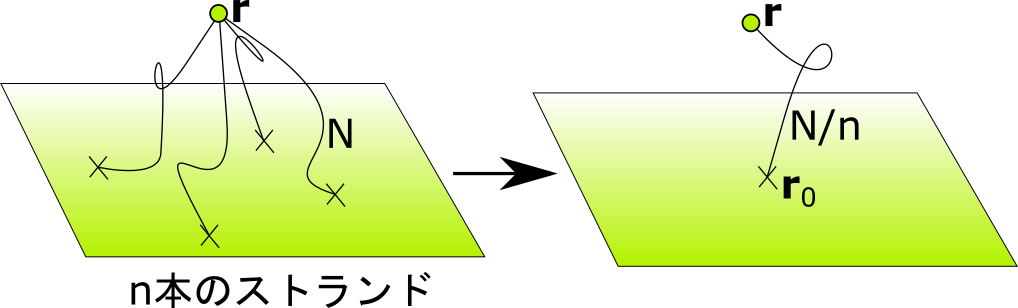
\includegraphics[width=\textwidth]{./fig/phantom-1.png}
% \end{figure}
% \end{block}
% \column{.48\textwidth}
% \begin{exampleblock}{内部の鎖が受ける変形}
% \begin{itemize}
% \item
% システム内部の鎖の末端はガウス分布
% \item
% 壁面に固定された末端からの変形が内部に伝達して、
% \end{itemize}
% \vspace{-5mm}
% \tiny
% \begin{align*}
% &G=\xi \nu k_BT \\
% &\begin{cases}
% \xi_{\infty} = 1-\dfrac{2}{f} \;\; \text{System}\sim \infty \\[8pt]
% \xi_{s} = \dfrac{f-1}{f+1} \;\; \text{Small Limit}
% \end{cases}
% \end{align*}
% \vspace{-7mm}
% \begin{figure}
% \centering
% 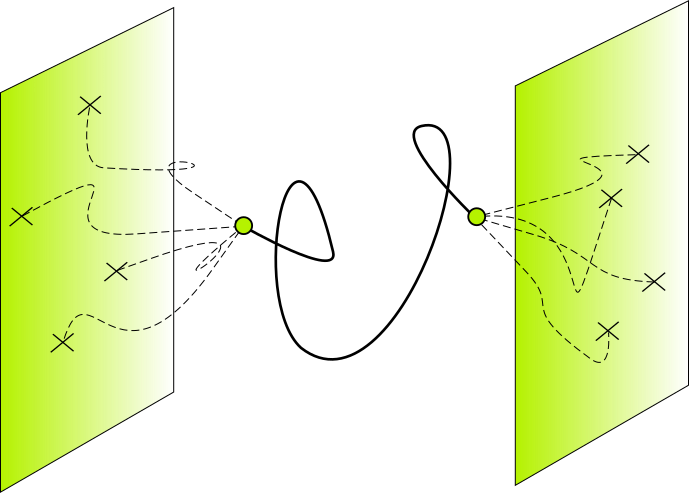
\includegraphics[width=0.6\textwidth]{./fig/phantom.png}
% \end{figure}
% \end{exampleblock}
% \end{columns}
% \end{frame}


% %%%%%%%%%%%%%%%%%%%%%%%%%%
% \begin{frame}
% \frametitle{ネットワークの分岐数の処理}
% 以下のようにノード番号を付与したネットワークを考えると、
% \begin{center}
% 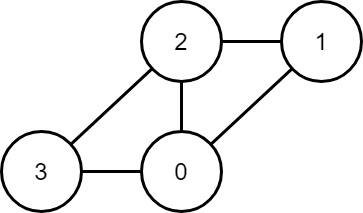
\includegraphics[width=4cm]{./fig/NW-4.png}
% \end{center}
% 隣接行列、および、次数行列は、
% \begin{align*}
% A = \left( 
% \begin{array}{cccc} 
% 0 & 1 & 1 & 1 \\ 
% 1 & 0 & 1 & 0 \\
% 1 & 1 & 0 & 1 \\
% 1 & 0 & 1 & 0 
% \end{array} 
% \right) 
% ,
% D = \left( 
% \begin{array}{cccc} 
% 3 & 0 & 0 & 0 \\ 
% 0 & 2 & 0 & 0 \\
% 0 & 0 & 3 & 0 \\
% 0 & 0 & 0 & 2 
% \end{array} 
% \right) 
% \end{align*}
% となる。
% \end{frame}
% %%%%%%%%%%%%%%%%%%%%%%%%%%
% \begin{frame}
% \frametitle{ラプラシアン行列}
% \begin{columns}[totalwidth=1\textwidth]
% \column{.48\textwidth}
% ラプラシアン行列は、隣接行列$A$と次数行列$D$により以下のように定義される。
% $$
% L \equiv D-A
% $$
% 4つのノードからなるネットワークの例であれば、
% $$
% L = \left( 
% \begin{array}{cccc} 
%  3 & -1 & -1 & -1 \\ 
% -1 &  2 & -1 & 0 \\
% -1 & -1 &  3 & -1 \\
% -1 &  0 & -1 & 2 
% \end{array} 
% \right) 
% $$
% となり、非負の固有値を有する。
% \column{.48\textwidth}
% グラフが非連結であるとき、%ラプラシアン行列の成分を
% 連結した成分ごとにブロック対角化できるので、固有値 0 の重複数がグラフの連結成分ブロックの総数となる。
% \begin{block}{「代数的連結性」}
% 「グラフが連結である場合、ラプラシアン行列の固有値 0 の重複数は 1」となる。\\
% 固有値を昇順にみた時、0 に次ぐ二番目の固有値がグラフの連結性の強さを示す指標となり、「代数的連結性」と呼ばれる。
% \end{block}
% \end{columns}
% \end{frame}

\end{document}
